%# Database File : Algebra-Or-Apolyth_Timh
%@ Database source: Mathematics
Απόλυτη τιμή ενός πραγματικού αριθμού $ a\in\mathbb{R} $ ονομάζεται η απόσταση του σημείου $ A $ του αριθμού από την αρχή $ O $ του άξονα των πραγματικών αριθμών. Συμβολίζεται με $ |a| $.
\begin{center}
\begin{tabular}{c >{\centering\arraybackslash}m{6cm}}
$ |a|=\begin{cases}
\begin{aligned}
a & \;,\;a\geq0\\
-a & \;,\;a<0
\end{aligned}
\end{cases} $  & 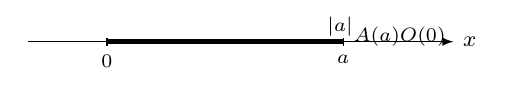
\begin{tikzpicture}
\draw[-latex] (-1,0) -- coordinate (x axis mid) (4.4,0) node[right,fill=white] {{\footnotesize $ x $}};
\draw (0,.5mm) -- (0,-.5mm) node[anchor=north,fill=white] {{\scriptsize $ 0 $}};
\draw (3,.5mm) -- (3,-.5mm) node[anchor=north,fill=white] {{\scriptsize $ a $}};
\draw[line width=.7mm] (0,0) -- (3,0);
\tkzText(1.5,.34){$ \overcbrace{\rule{28mm}{0mm}}^{{\scriptsize |a|}} $}
\tkzDefPoint(3,0){A}
\tkzDrawPoint(A)
\tkzLabelPoint[above right](A){{\scriptsize $A(a)$}}
\tkzDrawPoint(0,0)
\tkzLabelPoint[above left](0,0){{\scriptsize $O(0)$}}
\end{tikzpicture}
\end{tabular} 
\end{center}
Η απόλυτη τιμή ενός θετικού αριθμού $ a $ είναι ίση με τον ίδιο τον αριθμό ενώ η απόλυτη τιμή ενός αρνητικού αριθμού $ a $ είναι ίση με τον αντίθετο του δηλαδή $ -a $.
%# End of file Algebra-Or-Apolyth_Timh